\documentclass[]{book}
\usepackage{lmodern}
\usepackage{amssymb,amsmath}
\usepackage{ifxetex,ifluatex}
\usepackage{fixltx2e} % provides \textsubscript
\ifnum 0\ifxetex 1\fi\ifluatex 1\fi=0 % if pdftex
  \usepackage[T1]{fontenc}
  \usepackage[utf8]{inputenc}
\else % if luatex or xelatex
  \ifxetex
    \usepackage{mathspec}
  \else
    \usepackage{fontspec}
  \fi
  \defaultfontfeatures{Ligatures=TeX,Scale=MatchLowercase}
\fi
% use upquote if available, for straight quotes in verbatim environments
\IfFileExists{upquote.sty}{\usepackage{upquote}}{}
% use microtype if available
\IfFileExists{microtype.sty}{%
\usepackage{microtype}
\UseMicrotypeSet[protrusion]{basicmath} % disable protrusion for tt fonts
}{}
\usepackage[margin=1in]{geometry}
\usepackage{hyperref}
\hypersetup{unicode=true,
            pdftitle={Escritura de libros con bookdown},
            pdfauthor={Fernández-Casal, R. y Cotos-Yáñez, T.R.},
            pdfborder={0 0 0},
            breaklinks=true}
\urlstyle{same}  % don't use monospace font for urls
\usepackage{natbib}
\bibliographystyle{apalike}
\usepackage{color}
\usepackage{fancyvrb}
\newcommand{\VerbBar}{|}
\newcommand{\VERB}{\Verb[commandchars=\\\{\}]}
\DefineVerbatimEnvironment{Highlighting}{Verbatim}{commandchars=\\\{\}}
% Add ',fontsize=\small' for more characters per line
\usepackage{framed}
\definecolor{shadecolor}{RGB}{248,248,248}
\newenvironment{Shaded}{\begin{snugshade}}{\end{snugshade}}
\newcommand{\KeywordTok}[1]{\textcolor[rgb]{0.13,0.29,0.53}{\textbf{#1}}}
\newcommand{\DataTypeTok}[1]{\textcolor[rgb]{0.13,0.29,0.53}{#1}}
\newcommand{\DecValTok}[1]{\textcolor[rgb]{0.00,0.00,0.81}{#1}}
\newcommand{\BaseNTok}[1]{\textcolor[rgb]{0.00,0.00,0.81}{#1}}
\newcommand{\FloatTok}[1]{\textcolor[rgb]{0.00,0.00,0.81}{#1}}
\newcommand{\ConstantTok}[1]{\textcolor[rgb]{0.00,0.00,0.00}{#1}}
\newcommand{\CharTok}[1]{\textcolor[rgb]{0.31,0.60,0.02}{#1}}
\newcommand{\SpecialCharTok}[1]{\textcolor[rgb]{0.00,0.00,0.00}{#1}}
\newcommand{\StringTok}[1]{\textcolor[rgb]{0.31,0.60,0.02}{#1}}
\newcommand{\VerbatimStringTok}[1]{\textcolor[rgb]{0.31,0.60,0.02}{#1}}
\newcommand{\SpecialStringTok}[1]{\textcolor[rgb]{0.31,0.60,0.02}{#1}}
\newcommand{\ImportTok}[1]{#1}
\newcommand{\CommentTok}[1]{\textcolor[rgb]{0.56,0.35,0.01}{\textit{#1}}}
\newcommand{\DocumentationTok}[1]{\textcolor[rgb]{0.56,0.35,0.01}{\textbf{\textit{#1}}}}
\newcommand{\AnnotationTok}[1]{\textcolor[rgb]{0.56,0.35,0.01}{\textbf{\textit{#1}}}}
\newcommand{\CommentVarTok}[1]{\textcolor[rgb]{0.56,0.35,0.01}{\textbf{\textit{#1}}}}
\newcommand{\OtherTok}[1]{\textcolor[rgb]{0.56,0.35,0.01}{#1}}
\newcommand{\FunctionTok}[1]{\textcolor[rgb]{0.00,0.00,0.00}{#1}}
\newcommand{\VariableTok}[1]{\textcolor[rgb]{0.00,0.00,0.00}{#1}}
\newcommand{\ControlFlowTok}[1]{\textcolor[rgb]{0.13,0.29,0.53}{\textbf{#1}}}
\newcommand{\OperatorTok}[1]{\textcolor[rgb]{0.81,0.36,0.00}{\textbf{#1}}}
\newcommand{\BuiltInTok}[1]{#1}
\newcommand{\ExtensionTok}[1]{#1}
\newcommand{\PreprocessorTok}[1]{\textcolor[rgb]{0.56,0.35,0.01}{\textit{#1}}}
\newcommand{\AttributeTok}[1]{\textcolor[rgb]{0.77,0.63,0.00}{#1}}
\newcommand{\RegionMarkerTok}[1]{#1}
\newcommand{\InformationTok}[1]{\textcolor[rgb]{0.56,0.35,0.01}{\textbf{\textit{#1}}}}
\newcommand{\WarningTok}[1]{\textcolor[rgb]{0.56,0.35,0.01}{\textbf{\textit{#1}}}}
\newcommand{\AlertTok}[1]{\textcolor[rgb]{0.94,0.16,0.16}{#1}}
\newcommand{\ErrorTok}[1]{\textcolor[rgb]{0.64,0.00,0.00}{\textbf{#1}}}
\newcommand{\NormalTok}[1]{#1}
\usepackage{longtable,booktabs}
\usepackage{graphicx,grffile}
\makeatletter
\def\maxwidth{\ifdim\Gin@nat@width>\linewidth\linewidth\else\Gin@nat@width\fi}
\def\maxheight{\ifdim\Gin@nat@height>\textheight\textheight\else\Gin@nat@height\fi}
\makeatother
% Scale images if necessary, so that they will not overflow the page
% margins by default, and it is still possible to overwrite the defaults
% using explicit options in \includegraphics[width, height, ...]{}
\setkeys{Gin}{width=\maxwidth,height=\maxheight,keepaspectratio}
\IfFileExists{parskip.sty}{%
\usepackage{parskip}
}{% else
\setlength{\parindent}{0pt}
\setlength{\parskip}{6pt plus 2pt minus 1pt}
}
\setlength{\emergencystretch}{3em}  % prevent overfull lines
\providecommand{\tightlist}{%
  \setlength{\itemsep}{0pt}\setlength{\parskip}{0pt}}
\setcounter{secnumdepth}{5}
% Redefines (sub)paragraphs to behave more like sections
\ifx\paragraph\undefined\else
\let\oldparagraph\paragraph
\renewcommand{\paragraph}[1]{\oldparagraph{#1}\mbox{}}
\fi
\ifx\subparagraph\undefined\else
\let\oldsubparagraph\subparagraph
\renewcommand{\subparagraph}[1]{\oldsubparagraph{#1}\mbox{}}
\fi

%%% Use protect on footnotes to avoid problems with footnotes in titles
\let\rmarkdownfootnote\footnote%
\def\footnote{\protect\rmarkdownfootnote}

%%% Change title format to be more compact
\usepackage{titling}

% Create subtitle command for use in maketitle
\newcommand{\subtitle}[1]{
  \posttitle{
    \begin{center}\large#1\end{center}
    }
}

\setlength{\droptitle}{-2em}

  \title{Escritura de libros con bookdown}
    \pretitle{\vspace{\droptitle}\centering\huge}
  \posttitle{\par}
    \author{Fernández-Casal, R. y Cotos-Yáñez, T.R.}
    \preauthor{\centering\large\emph}
  \postauthor{\par}
      \predate{\centering\large\emph}
  \postdate{\par}
    \date{2018-10-25}

\usepackage{booktabs}
\usepackage{amsthm}
\ifxetex
  \usepackage{polyglossia}
  \setmainlanguage{spanish}

  % Tabla en lugar de cuadro
  \gappto\captionsspanish{\renewcommand{\tablename}{Tabla}  
          \renewcommand{\listtablename}{Índice de tablas}}

\else
  \usepackage[spanish,es-tabla]{babel}
  % Para los acentos (xelatex no lo necesita)
\fi
\makeatletter
\def\thm@space@setup{%
  \thm@preskip=8pt plus 2pt minus 4pt
  \thm@postskip=\thm@preskip
}
\makeatother

\usepackage{amsthm}
\newtheorem{theorem}{Teorema}[chapter]
\newtheorem{lemma}{Lema}[chapter]
\theoremstyle{definition}
\newtheorem{definition}{Definición}[chapter]
\newtheorem{corollary}{Corolario}[chapter]
\newtheorem{proposition}{Proposición}[chapter]
\theoremstyle{definition}
\newtheorem{example}{Ejemplo}[chapter]
\theoremstyle{definition}
\newtheorem{exercise}{Ejercicio}[chapter]
\theoremstyle{remark}
\newtheorem*{remark}{Nota: }
\newtheorem*{solution}{Solución}
\let\BeginKnitrBlock\begin \let\EndKnitrBlock\end
\begin{document}
\maketitle

{
\setcounter{tocdepth}{1}
\tableofcontents
}
\chapter*{Prólogo}\label{prologo}
\addcontentsline{toc}{chapter}{Prólogo}

Este libro es una pequeña guía sobre como emplear el paquete
\texttt{bookdown} de R para la escritura de libros, incluyendo algunos
detalles de configuración para la escritura en otros idiomas distintos
del inglés (castellano, galego,\ldots{}).

Este mismo libro ha sido escrito en
\href{http://rmarkdown.rstudio.com}{R-Markdown} empleando el paquete
\href{https://bookdown.org/yihui/bookdown/}{\texttt{bookdown}} y está
disponible en el repositorio Github:
\href{https://github.com/rubenfcasal/bookdown_intro}{rubenfcasal/bookdown\_intro}.

Para generar el libro (compilar) puede ser recomendable instalar la
última versión de
\href{(https://www.rstudio.com/products/rstudio/download/)}{RStudio} y
la versión de desarrollo de \texttt{bookdown} disponible en
\href{https://github.com/rstudio/bookdown}{Github}. En la Sección
\ref{requisitos} se detallan los requisitos necesarios.

\begin{flushleft}
\includegraphics{images/by-sa-88x31} \end{flushleft}

Esta obra está bajo una licencia de
\href{https://creativecommons.org/licenses/by-sa/4.0/deed.es}{Creative
Commons Reconocimiento-CompartirIgual 4.0 Internacional}.

\chapter{Introducción}\label{intro}

El paquete \texttt{bookdown} \citep{R-bookdown} de R \citep{R-base}
permite escribir libros empleando \href{http://rmarkdown.rstudio.com}{R
Markdown} de forma fácil. Sin preocuparse mucho por los detalles de
composición se pueden crear libros en distintos formatos (HTML / LaTeX /
PDF / EPUB / \ldots{}). Además de permitir emplear las extensiones
Markdown de Pandoc (notas al pie de página, tablas, citas, ecuaciones
LaTeX, \ldots{}), se pueden emplear extensiones Markdown para libros
(leyendas de figuras y tablas, numeración y referencias cruzadas de
figuras / tablas / secciones / ecuaciones / teoremas / ejemplos /
\ldots{}, widgets HTML, \ldots{}).

Este libro es una pequeña guía para la escritura de libros con este
paquete (incluyendo algunos detalles para la escritura en otros idiomas
distintos del inglés), pero se supone que el lector ya tiene
conocimientos de RMarkdown. En el Apéndice \ref{rmarkdown} se incluye
algo de información sobre este lenguaje, pero la recomendación sería
buscar fuentes adicionales de información si no se conoce, empezando por
la web \url{http://rmarkdown.rstudio.com/} y las fuentes descritas en
dicho apéndice. También recomendamos consultar fuentes externas para
obtener documentación detallada sobre los distintos temas, como por
ejemplo los libros (disponibles de forma gratuita en línea):

\begin{itemize}
\item
  \citet{R-bookdown} : Authoring Books and Technical Documents with R
  Markdown, \url{https://bookdown.org/yihui/bookdown/}.
\item
  \citet{xie2018r} : R Markdown: The Definitive Guide,
  \url{https://bookdown.org/yihui/rmarkdown/}.
\end{itemize}

Ejemplos de este tipo de libros\footnote{Los libros de Hadley
  \href{http://adv-r.had.co.nz}{Advanced R} y
  \href{http://r-pkgs.had.co.nz}{R packages} serían ejemplos con una
  versión ``preliminar'' de este paquete.} se tienen en
\url{https://bookdown.org} (el listado completo está disponible
\href{https://bookdown.org/home/archive/}{aquí}). Además de este, otros
libros en castellano que se puede utilizar como ejemplo son:

\begin{itemize}
\item
  \href{https://rubenfcasal.github.io/simbook}{Prácticas de Simulación},
  disponible en el repositorio de GitHub
  \href{https://github.com/rubenfcasal/simbook}{rubenfcasal/simbook}
  (\href{https://github.com/rubenfcasal/simbook/archive/master.zip}{Zip}).
\item
  \href{https://www.datanalytics.com/libro_r/index.html}{R para
  profesionales de los datos: una introducción}.
\end{itemize}

Si ya se dispone de contenido en otros formatos sobre el tema del libro,
el primer paso sería su conversión a formato RMarkdown. Para ello se
puede emplear Pandoc (ver Apéndice \ref{pandoc}), siguiendo los pasos
descritos en la Sección \ref{conversion}.

\section{Requisitos}\label{requisitos}

\begin{enumerate}
\def\labelenumi{\arabic{enumi}.}
\item
  Disponer de una versión reciente de RStudio.
  \href{https://www.rstudio.com/products/rstudio/download/}{Descargar la
  última versión} si la versión actual es anterior a la 1.0.0.
\item
  Instalar el paquete \texttt{bookdown} de R:

\begin{Shaded}
\begin{Highlighting}[]
\CommentTok{# stable version on CRAN}
\KeywordTok{install.packages}\NormalTok{(}\StringTok{'bookdown'}\NormalTok{)}
\CommentTok{# or development version on GitHub}
\CommentTok{# devtools::install_github('rstudio/bookdown')}
\end{Highlighting}
\end{Shaded}
\item
  Para compilar los libros en pdf \texttt{bookdown} emplea XeLaTeX. En
  windows es recomendable instalar
  \href{https://miktex.org/download}{MiKTeX}, o actualizarlo (ejecutando
  MiKTeX Update) si ya está instalado. En Mac OS X se puede instalar
  \href{http://www.tug.org/mactex/}{MacTeX} y en Linux
  \href{http://www.tug.org/texlive}{TeXLive}\footnote{Aunque el autor
    del paquete \texttt{bookdown} recomienda instalar
    \href{https://yihui.name/tinytex}{TinyTeX}.}.
\end{enumerate}

\section{Primeros pasos}\label{primeros-pasos}

Si se emplea RStudio (recomendado), lo más cómodo sería crear un
proyecto nuevo empleando el menú \emph{File \textgreater{} New Project
\textgreater{} New Directory \textgreater{} Book project using
bookdown}. Alternativamente se podría usar como plantilla algún libro
publicado (este se puede descargar
\href{https://github.com/rubenfcasal/bookdown_intro/archive/master.zip}{aquí}).
Por ejemplo, el proyecto que crea por defecto RStudio está disponible en
el repositorio de GitHub
\href{https://github.com/rstudio/bookdown-demo}{rstudio/bookdown-demo} y
se puede descargar como fichero
\href{https://github.com/rstudio/bookdown-demo/archive/master.zip}{Zip}.
Posteriormente se pueden ir modificando (añadiendo o eliminando) los
ficheros \emph{.Rmd} correspondientes a los distintos capítulos.

Si se abre el proyecto en RStudio, se puede compilar empleando el boton
\emph{Build Book}\footnote{Alternativamente se puede ejecutar la función
  \texttt{render\_book()} en el directorio del proyecto} en la pestaña
\emph{Build}. Por defecto se generará el libro (en los distintos
formatos) en la carpeta \emph{\_book} y al terminar se abrirá
automáticamente la versión HTML. El libro se generará (de forma
simultánea en los formatos deseados) a partir de una serie de documentos
R Markdown, cada uno correspondiente a un capítulo.

\textbf{Nota}: Si se produce un error, puede ser necesario\footnote{Esto
  debería hacerse automáticamente si se incluye la opción
  \texttt{delete\_merged\_file:\ true} en el fichero de configuración
  \emph{\_bookdown.yml}.} eliminar manualmente los ficheros de salida
(e.g.\\
\emph{book\_filename.Rmd} o \emph{book\_filename.md}) para poder volver
a compilar.

\section{Estructura del libro}\label{estructura-del-libro}

La estructura del libro se corresponde con un conjunto de directorios y
ficheros, los principales serían:

\begin{itemize}
\item
  Un fichero inicial de RMarkdown \emph{index.Rmd} con diferentes
  configuraciones generales (título, autor, fecha, \ldots{}) y donde se
  puede incluir un prólogo/preámbulo/prefacio.
\item
  Un fichero de RMarkdown \emph{.Rmd} para cada capítulo, definido por
  el título de primer nivel \texttt{\#}. Los capítulos se ordenarán
  siguiendo el orden alfabético de los nombres de los ficheros\footnote{Evitar
    espacios (y acentos) en los nombres de los ficheros de los
    capítulos.}.
\item
  Archivo \emph{\_bookdown.yml} de configuración donde se espefican
  parámetros opcionales para la compilación del libro.
\item
  Archivo \emph{\_output.yml} de configuración con las opciones del
  formato de salida.
\item
  Archivos \emph{style.css} y \emph{preamble.tex} con especificaciones
  de las opciones de estilo de los libros en formato HTML e LaTeX,
  respectivamente.
\item
  Archivo \emph{book.bib} con las referencias biliográficas en formato
  BibTeX.
\end{itemize}

Se pueden incluir directorios adicionales, por ejemplo una carpeta
\emph{images} que contenga las imágenes estáticas y una carpeta de
\emph{data} con los archivos de datos a usar.

\chapter{Archivos de configuración}\label{archivos-de-configuracion}

Nos puede interesar modificar el encabezado de \emph{index.Rmd} y un par
de archivos \href{https://en.wikipedia.org/wiki/YAML}{YAML} de
configuración (ver Sección \ref{yaml} para más detalles sobre este
formato).

\section{\texorpdfstring{Encabezado de \emph{index.Rmd} y archivo
\emph{\_output.yml}}{Encabezado de index.Rmd y archivo \_output.yml}}\label{encabezado-de-index.rmd-y-archivo-_output.yml}

La cabecera YAML del primer archivo \emph{.Rmd} del libro se puede
utilizar para configurar distintas opciones:

\begin{Shaded}
\begin{Highlighting}[]
\OtherTok{--- }
\FunctionTok{title:}\AttributeTok{ }\StringTok{"A Minimal Book Example"}
\FunctionTok{author:}\AttributeTok{ }\StringTok{"Yihui Xie"}
\FunctionTok{date:}\AttributeTok{ }\StringTok{"2018-10-25"}
\FunctionTok{site:}\AttributeTok{ bookdown::bookdown_site}
\FunctionTok{output:}\AttributeTok{ bookdown::gitbook}
\FunctionTok{documentclass:}\AttributeTok{ book}
\FunctionTok{bibliography:}\AttributeTok{ }\KeywordTok{[}\NormalTok{book.bib}\KeywordTok{,}\NormalTok{ packages.bib}\KeywordTok{]}
\FunctionTok{biblio-style:}\AttributeTok{ apalike}
\FunctionTok{link-citations:}\AttributeTok{ yes}
\FunctionTok{github-repo:}\AttributeTok{ rstudio/bookdown-demo}
\FunctionTok{description:}\AttributeTok{ }\StringTok{"This is a minimal example of using the bookdown package to write a book.}
\StringTok{The output format for this example is bookdown::gitbook."}
\OtherTok{---}
\end{Highlighting}
\end{Shaded}

Obviamente cambiaremos el título, el nombre del autor y la descripción
(también nos podrá interesar cambiar las opciones de bibliografía, ver
Sección \ref{biblio}, o las del repositorio GitHub, ver Sección
\ref{github}). Por ejemplo, se puede acceder al fichero \emph{index.Rmd}
de este libro
\href{https://github.com/rubenfcasal/bookdown_intro/raw/master/index.Rmd}{aquí}
.

Aunque se pueden especificar en esta cabecera otras opciones
relacionadas con Pandoc, como por ejemplo opciones del formato de
salida:

\begin{Shaded}
\begin{Highlighting}[]
\OtherTok{---}
\FunctionTok{output:}
  \FunctionTok{bookdown:}\AttributeTok{:gitbook:}
    \FunctionTok{split_by:}\AttributeTok{ }\StringTok{"section"}\ErrorTok{       # Páginas por secciones (en lugar de capítulos)}
    \FunctionTok{split_bib:}\AttributeTok{ no             }\CommentTok{# No se muestra bibliografía al final de cada página}
    \FunctionTok{lib_dir:}\AttributeTok{ }\StringTok{"book_assets"}
  \FunctionTok{bookdown:}\AttributeTok{:pdf_book:}
    \FunctionTok{keep_tex:}\AttributeTok{ yes}
\OtherTok{---}
\end{Highlighting}
\end{Shaded}

Normalmente estableceremos las opciones del formato de salida en el
archivo de configuración YAML \emph{\_output.yml}. Por defecto se generá
el libro en formato HTML (con las opciones de
\texttt{bookdown::gitbook()}), en formato PDF a través de LaTeX
(\texttt{bookdown::pdf\_book()}) y en formato EPUB
(\texttt{bookdown::epub\_book()}). En este archivo también nos
interesará cambiar algunas de las opciones por defecto:

\begin{Shaded}
\begin{Highlighting}[]
\FunctionTok{bookdown:}\AttributeTok{:gitbook:}
  \FunctionTok{css:}\AttributeTok{ style.css}
  \FunctionTok{config:}
    \FunctionTok{toc:}
      \FunctionTok{before:}\AttributeTok{ |}
\NormalTok{        <li><a href=}\StringTok{"./"}\NormalTok{>A Minimal Book Example</a></li>}
      \FunctionTok{after:}\AttributeTok{ |}
        \FunctionTok{<li><a href="https:}\AttributeTok{//github.com/rstudio/bookdown" target="blank">Published with bookdown</a></li>}
    \FunctionTok{edit:}\AttributeTok{ https://github.com/rstudio/bookdown-demo/edit/master/%s}
    \FunctionTok{download:}\AttributeTok{ }\KeywordTok{[}\StringTok{"pdf"}\KeywordTok{,} \StringTok{"epub"}\KeywordTok{]}
\FunctionTok{bookdown:}\AttributeTok{:pdf_book:}
  \FunctionTok{includes:}
    \FunctionTok{in_header:}\AttributeTok{ preamble.tex}
  \FunctionTok{latex_engine:}\AttributeTok{ xelatex}
  \FunctionTok{citation_package:}\AttributeTok{ natbib}
  \FunctionTok{keep_tex:}\AttributeTok{ yes}
\FunctionTok{bookdown:}\AttributeTok{:epub_book: default}
\end{Highlighting}
\end{Shaded}

Por lo menos en el formato HTML \texttt{bookdown::gitbook}, el título
del documento en la parte superior de la tabla de contenido. El fichero
\href{https://github.com/rubenfcasal/bookdown_intro/blob/master/_output.yml}{\emph{\_output.yml}}
de este libro es:

\begin{Shaded}
\begin{Highlighting}[]
\FunctionTok{bookdown:}\AttributeTok{:gitbook:}
  \FunctionTok{css:}\AttributeTok{ style.css}
  \FunctionTok{config:}
    \FunctionTok{toc:}
      \FunctionTok{before:}\AttributeTok{ |}
\NormalTok{        <li><a href=}\StringTok{"./"}\NormalTok{>Escritura de libros con bookdown</a></li>}
      \FunctionTok{after:}\AttributeTok{ |}
        \FunctionTok{<li><a href="https:}\AttributeTok{//github.com/rstudio/bookdown" target="blank">Publicado con bookdown</a></li>}
    \FunctionTok{edit:}\AttributeTok{ https://github.com/rubenfcasal/bookdown_intro/edit/master/%s      }\CommentTok{# Si se publica con GitHub Pages...}
    \FunctionTok{download:}\AttributeTok{ }\StringTok{"pdf"}\ErrorTok{                                                         # Link de descarga en pdf}
\FunctionTok{bookdown:}\AttributeTok{:pdf_book:}
  \FunctionTok{includes:}
    \FunctionTok{in_header:}\AttributeTok{ preamble.tex}
  \FunctionTok{latex_engine:}\AttributeTok{ xelatex}
  \FunctionTok{citation_package:}\AttributeTok{ natbib}
  \FunctionTok{keep_tex:}\AttributeTok{ yes}
\end{Highlighting}
\end{Shaded}

Más detalles sobre las opciones de salida en el
\href{https://bookdown.org/yihui/bookdown/output-formats.html}{libro de
bookdown}. Otros ejemplos en castellano de
\href{https://github.com/rubenfcasal/simbook/raw/master/index.Rmd}{\emph{index.Rmd}}
y
\href{https://github.com/rubenfcasal/simbook/blob/master/_output.yml}{\emph{\_output.yml}}.

\section{\texorpdfstring{Archivo
\emph{\_bookdown.yml}}{Archivo \_bookdown.yml}}\label{archivo-_bookdown.yml}

El fichero de configuración por defecto es:

\begin{Shaded}
\begin{Highlighting}[]
\FunctionTok{book_filename:}\AttributeTok{ }\StringTok{"bookdown-demo"}
\FunctionTok{language:}
  \FunctionTok{ui:}
    \FunctionTok{chapter_name:}\AttributeTok{ }\StringTok{"Chapter "}
\FunctionTok{delete_merged_file:}\AttributeTok{ true    }
\end{Highlighting}
\end{Shaded}

Por ejemplo, nos interesará cambiar el nombre del fichero y, si se trata
de un libro en castellano (galego, \ldots{}), el encabezado de los
títulos de los capítulos. Además nos puede interesar cambiar los
encabezados de algunos componentes como figuras y tablas, siguiendo las
instrucciones de la
\href{https://bookdown.org/yihui/bookdown/internationalization.html}{Sección
4.5} del libro de bookdown. Por ejemplo en este libro se emplea:

\begin{Shaded}
\begin{Highlighting}[]
\FunctionTok{book_filename:}\AttributeTok{ }\StringTok{'bookdown_intro'}
\FunctionTok{output_dir:}\AttributeTok{ docs}
\FunctionTok{new_session:}\AttributeTok{ no}
\FunctionTok{language:}
  \FunctionTok{label:}
    \FunctionTok{fig:}\AttributeTok{ }\StringTok{'Figura '}
    \FunctionTok{tab:}\AttributeTok{ }\StringTok{'Tabla '}
    \FunctionTok{eq:}\AttributeTok{ }\StringTok{'Ecuación '}
    \FunctionTok{thm:}\AttributeTok{ }\StringTok{'Teorema '}
    \FunctionTok{lem:}\AttributeTok{ }\StringTok{'Lema '}
    \FunctionTok{def:}\AttributeTok{ }\StringTok{'Definición '}
    \FunctionTok{cor:}\AttributeTok{ }\StringTok{'Corolario '}
    \FunctionTok{prp:}\AttributeTok{ }\StringTok{'Proposición '}
    \FunctionTok{exm:}\AttributeTok{ }\StringTok{'Ejemplo '}
    \FunctionTok{exr:}\AttributeTok{ }\StringTok{'Ejercicio '}
    \FunctionTok{proof:}\AttributeTok{ }\StringTok{'Demostración. '}
    \FunctionTok{remark:}\AttributeTok{ }\StringTok{'Nota: '}
    \FunctionTok{solution:}\AttributeTok{ }\StringTok{'Solución. '}
  \FunctionTok{ui:}
    \FunctionTok{chapter_name:}\AttributeTok{ }\StringTok{'Capítulo '}
\FunctionTok{delete_merged_file:}\AttributeTok{ yes}
\end{Highlighting}
\end{Shaded}

y puede ser descargado
\href{https://github.com/rubenfcasal/bookdown_intro/raw/master/_bookdown.yml}{aquí}.
Además se modificó \emph{preamble.tex} para configurar LaTeX para
castellano, añadiendo:

\begin{Shaded}
\begin{Highlighting}[]
\FunctionTok{\textbackslash{}ifxetex}
  \BuiltInTok{\textbackslash{}usepackage}\NormalTok{\{}\ExtensionTok{polyglossia}\NormalTok{\}}
  \FunctionTok{\textbackslash{}setmainlanguage}\NormalTok{\{spanish\}}
  \CommentTok{% Tabla en lugar de cuadro}
  \FunctionTok{\textbackslash{}gappto\textbackslash{}captionsspanish}\NormalTok{\{}\FunctionTok{\textbackslash{}renewcommand}\NormalTok{\{}\ExtensionTok{\textbackslash{}tablename}\NormalTok{\}\{Tabla\}  }
          \FunctionTok{\textbackslash{}renewcommand}\NormalTok{\{}\ExtensionTok{\textbackslash{}listtablename}\NormalTok{\}\{Índice de tablas\}\}}
\FunctionTok{\textbackslash{}else}
  \BuiltInTok{\textbackslash{}usepackage}\NormalTok{[spanish,es-tabla]\{}\ExtensionTok{babel}\NormalTok{\}}
\FunctionTok{\textbackslash{}fi}
\end{Highlighting}
\end{Shaded}

Otras opciones permitirían cambiar el orden de los ficheros \emph{.Rmd}
(\texttt{rmd\_files:}) , o establecer y configurar la sesión de R donde
se evalúa el código. Por ejemplo:

\begin{Shaded}
\begin{Highlighting}[]
\FunctionTok{new_session:}\AttributeTok{ yes                                    }\CommentTok{# Cada capítulo en una nueva sesión}
\FunctionTok{before_chapter_script:}\AttributeTok{ }\KeywordTok{[}\StringTok{"script1.R"}\KeywordTok{,} \StringTok{"script2.R"}\KeywordTok{]}\AttributeTok{   }\CommentTok{# Ejecutar código antes de los capítulos}
\FunctionTok{after_chapter_script:}\AttributeTok{ }\StringTok{"script3.R"}\ErrorTok{                   # y después.}
\end{Highlighting}
\end{Shaded}

Más detalles de las opciones de configuración en el
\href{https://bookdown.org/yihui/bookdown/configuration.html\#configuration}{libro
de bookdown}.

\chapter{Componentes}\label{componentes}

\section{Introducción}\label{introduccion}

Para la elaboración de contenido se pueden emplear las componentes de
RMarkdown descritas en el Apéndice \ref{rmarkdown}, incluyendo la
sintaxis de Markdown (Sección \ref{markdown}) y la inclusión de bloques
de código en R (Sección \ref{codigormd}). Pero como se comenta en este
Apéndice, RMarkdown admite extensiones adicionales (proporcionadas por
Pandoc), que pueden ser de utilidad en la escritura de un libro. Por
ejemplo, se pueden añadir sub\textsubscript{índices} y
super\textsuperscript{índices} con
\texttt{sub\textasciitilde{}índices\textasciitilde{}} y
\texttt{super\^{}índices\^{}}, notas al pie con
\texttt{\^{}{[}texto{]}}, ecuaciones y referencias bibliográficas.

El paquete \texttt{bookdown} proporciona extensiones adicionales de la
sistaxis de RMarkdown especialmente diseñadas para la escritura de
libros (ver p.e. la
\href{https://bookdown.org/yihui/bookdown/markdown-extensions-by-bookdown.html}{Sección
2.2} del libro de bookdown), además el comportamiento de algunos
resultados cambia al renderizar con este paquete.

El las siguientes secciones se mostrarán algunas de estas extensiones de
RMarkdown y de \texttt{bookdown} (en el
\href{https://bookdown.org/yihui/bookdown/markdown-extensions-by-bookdown.html}{Capítulo
2} del libro de bookdown se detallan todas las extensiones
\texttt{bookdown}, incluyendo referencias de texto, bloques
personalizados, HTML widgets, páginas web y aplicaciones Shiny).

\section{Secciones y cabeceras}\label{secciones-y-cabeceras}

Como ya se comentó, en el fichero de RMarkdown \texttt{.Rmd} de cada
capítulo, este está definido por el título de primer nivel (e.g.
\texttt{\#\ Título}; ver Sección \ref{markdown} para la sintaxis de los
distintos niveles de cabeceras), por lo que sólo debería haber uno.
Además, al renderizar con \texttt{bookdown} los capítulos y secciones se
numeran automáticamente, siguiendo el orden alfabético de los ficheros.

Si no se desea numerar algún capítulo o sección, habrá que anádir
\texttt{\{-\}} a continuación del correspondiente título (por ejemplo,
en el archivo \emph{index.Rmd} se incluyó \texttt{\#\ Prólogo\ \{-\}}).

Para referenciar un capítulo o sección, se puede añadir una etiqueta de
la forma \texttt{\{\#etiqueta\}} a continuación del correspondiente
título, después se podrá referenciar en el texto empleando
\texttt{\textbackslash{}@ref(etiqueta)}, que al renderizar producirá un
enlace con la correspondiente numeración (más detalles en la
\href{https://bookdown.org/yihui/bookdown/cross-references.html}{Sección
2.6} del libro de bookdown).

Adicionalmente hay dos tipos especiales de cabeceras de primer nivel que
pueden ser empleadas en \texttt{bookdown}:

\begin{itemize}
\item
  \texttt{\#\ (PARTE)\ Titulo\ de\ la\ Parte\ \{-\}}: para separar
  capítulos en partes.
\item
  \texttt{\#\ (APPENDIX)\ Apéndices\ \{-\}}: para crear apéndices. Los
  capítulos posteriores se tratarán como apéndices y se numerarán
  alfabeticamente (A, B, C, \ldots{}).,
\end{itemize}

\section{Figuras y tablas}\label{figuras-y-tablas}

En la Sección \ref{opcodigo} se comentan algunas opciones de los bloques
de código que pueden ser de utilidad para las figuras (algunas se pueden
establecer en \emph{\_output.yml}, ver Sección \ref{yaml}). Por ejemplo,
se puede establecer la opción \texttt{fig.cap} para incluir una leyenda
(sin incluir sintaxis Markdown, salvo que se utilicen referencias de
texto). En ese caso la gráfica se colocará en un entorno de figura
(flotante en PDF/LaTeX\footnote{Se puede ajustar las posición empleando
  la opción de \texttt{fig.pos} (por ejemplo,
  \texttt{fig.pos\ =\ \textquotesingle{}!htb\textquotesingle{}}).}), que
se etiquetará y numerará automáticamente.

Para referenciar una figura, habrá que añadir el prefijo \texttt{fig:}
al nombre del bloque de código. Por ejemplo, la referencia a una figura
en un bloque con nombre \texttt{foo} será
\texttt{\textbackslash{}@ref(fig:foo)}.

Para incluir imágenes estáticas, en lugar de emplear la sintaxis
habitual de markdown (e.g. \texttt{!{[}{]}(rmarkdown.png)}), se puede
llamar a la función \texttt{knitr::include\_graphics()} en un bloque de
código para poder emplear las extensiones \texttt{bookdown}. Por
ejemplo, la figura \ref{fig:rmarkdown} se incluyó con el siguiente
código:

\begin{Shaded}
\begin{Highlighting}[]
\NormalTok{```\{r rmarkdown, echo=FALSE, out.width='30%', fig.align='center', fig.cap='Logo de rmarkdown (desde archivo PNG).'\}}
\NormalTok{knitr::include_graphics("images/rmarkdown.png")}
\NormalTok{```}
\end{Highlighting}
\end{Shaded}

\begin{figure}

{\centering 
\includegraphics[width=0.3\linewidth]{images/rmarkdown} 

}

\caption{Logo de rmarkdown (desde archivo PNG).}\label{fig:rmarkdown}
\end{figure}

Además puede ser recomendable guardar estas imágenes en un subdirectorio
(\emph{images} en el caso de este libro). En la
\href{https://bookdown.org/yihui/bookdown/figures.html}{Sección 2.4} del
libro de bookdown se tienen más detalles sobre las Figuras.

Las tablas se comportan de forma similar. Si se emplea la función
\texttt{knitr::ktable()} para incluir tablas, como se describe en la
Sección \ref{tablas}, estas se colocarán en un entorno de tabla
(flotante en PDF/LaTeX), y se etiquetarán y numerarán automáticamente.
Para referenciarlas, habrá que añadir el prefijo \texttt{tab:} al nombre
del bloque de código (e.g. \texttt{\textbackslash{}@ref(tab:foo)}). Más
detalles en la
\href{https://bookdown.org/yihui/bookdown/tables.html}{Sección 2.5} del
libro de bookdown.

\section{Ecuaciones}\label{ecuaciones}

RMarkdown permite incluir expresiones matemáticas en formato LateX:

\begin{itemize}
\item
  En linea escribiendo la expresión latex entre dos símbolos de dolar,
  por ejemplo
  \texttt{\$\textbackslash{}alpha,\ \textbackslash{}beta,\ \textbackslash{}gamma,\ \textbackslash{}delta\$}
  resultaría en \(\alpha, \beta, \gamma, \delta\).
\item
  En formato ecuación empleando dos pares de símbolos de dolar. Por
  ejemplo:

\begin{verbatim}
$$\Theta = \begin{pmatrix}\alpha & \beta\\
\gamma & \delta
\end{pmatrix}$$
\end{verbatim}

  resultaría en: \[\Theta = \begin{pmatrix}\alpha & \beta\\
  \gamma & \delta
  \end{pmatrix}\]
\end{itemize}

Adicionalmente en \texttt{bookdown} se pueden incluir ecuaciones
numeradas (empleando directamente sintaxis LaTeX), que pueden ser
referenciadas posteriormente. Por ejemplo:

\begin{Shaded}
\begin{Highlighting}[]
\KeywordTok{\textbackslash{}begin}\NormalTok{\{}\ExtensionTok{equation}\NormalTok{\}}\SpecialStringTok{ }
\SpecialStringTok{  f}\SpecialCharTok{\textbackslash{}left}\SpecialStringTok{(k}\SpecialCharTok{\textbackslash{}right}\SpecialStringTok{) = }\SpecialCharTok{\textbackslash{}binom}\SpecialStringTok{\{n\}\{k\} p^k}\SpecialCharTok{\textbackslash{}left}\SpecialStringTok{(1-p}\SpecialCharTok{\textbackslash{}right}\SpecialStringTok{)^\{n-k\}}
\SpecialStringTok{  (}\SpecialCharTok{\textbackslash{}#}\SpecialStringTok{eq:ecuacion1)}
\SpecialCharTok{\textbackslash{}end}
\end{Highlighting}
\end{Shaded}

produce la siguiente ecuación \eqref{eq:ecuacion1}:

\begin{equation}
f\left(k\right)=\binom{n}{k}p^k\left(1-p\right)^{n-k} \label{eq:ecuacion1}
\end{equation}

que puede ser referenciada con
\texttt{\textbackslash{}@ref(eq:ecuacion1)} (más detalles
\href{https://bookdown.org/yihui/bookdown/markdown-extensions-by-bookdown.html\#equations}{aquí}).

\section{Referencias bibliográficas}\label{biblio}

RMarkdown también admite bibliografía en distintos formatos, ver p.e.
\url{https://rmarkdown.rstudio.com/authoring_bibliographies_and_citations.html}.
Por defecto \texttt{bookdown} emplea referencias bibliográficas en
formato BibTeX (lo que se describe con detalle
\href{https://bookdown.org/yihui/bookdown/citations.html}{aquí}). Para
especificar uno o más archivos de bibliografía \emph{.bib}, se usa el
campo \texttt{bibliography} en el fichero \emph{Index.Rmd}. Por defecto
es de la forma:

\begin{Shaded}
\begin{Highlighting}[]
\OtherTok{---}
\FunctionTok{bibliography:}\AttributeTok{ }\KeywordTok{[}\StringTok{"book.bib"}\KeywordTok{,} \StringTok{"packages.bib"}\KeywordTok{]}
\FunctionTok{biblio-style:}\AttributeTok{ }\StringTok{"apalike"}
\FunctionTok{link-citations:}\AttributeTok{ true}
\OtherTok{---}
\end{Highlighting}
\end{Shaded}

Por ejemplo, una entrada de BibTeX sería:

\begin{Shaded}
\begin{Highlighting}[]
\VariableTok{@book}\NormalTok{\{}\OtherTok{xie2016bookdown}\NormalTok{,}
  \DataTypeTok{title}\NormalTok{=\{Bookdown: Authoring Books and Technical Documents with R Markdown\},}
  \DataTypeTok{author}\NormalTok{=\{Xie, Yihui\},}
  \DataTypeTok{year}\NormalTok{=\{2016\},}
  \DataTypeTok{publisher}\NormalTok{=\{Chapman and Hall/CRC\}}
\NormalTok{\}}
\end{Highlighting}
\end{Shaded}

Si se añade al fichero \emph{book.bib} podemos referenciarla en el texto
empleando\footnote{En RStudio se puede instalar el
  ``\href{https://rstudio.github.io/rstudioaddins/}{Addin}''
  \href{https://github.com/crsh/citr}{\texttt{citr}} para insertar citas
  a referencias bibliográficas en formato BibTeX.}
\texttt{@xie2016bookdown} o \texttt{{[}@xie2016bookdown{]}}, resultando
\citet{xie2016bookdown} o \citep{xie2016bookdown}.

Además, en el fichero \emph{index.Rmd} se incluye por defecto el
siguiente código:

\begin{verbatim}
# automatically create a bib database for R packages
knitr::write_bib(c(.packages(), 'bookdown', 'knitr', 'rmarkdown'), 'packages.bib')
\end{verbatim}

que genera automáticamente el archivo \emph{packages.bib} con las
referencias bibliográficas de los paquetes especificados (puede
interesar añadir los paquetes empleados). En el texto RMarkdown estas
referencias se incluyen con \texttt{@R-paquete} (o
\texttt{{[}@R-paquete{]}}), y la referencia a R \citep{R-base} con
\texttt{{[}@R-base{]}}.

Pandoc generará el listado de referencias al final del documento, por lo
que habría que insertar una última sección
\texttt{\#\ Bibliografía\ \{-\}} al generar el libro en dormato HTML (en
PDF se hará automáticamente al emplear LaTeX). Si además de HTML se
empleán otros formatos, se puede añadir el código:

\begin{Shaded}
\begin{Highlighting}[]
\BaseNTok{`r if (knitr:::is_html_output()) '# Bibliografía \{-\}'`}
\end{Highlighting}
\end{Shaded}

al final del documento.

\section{Entornos}\label{entornos}

El paquete \texttt{bookdown} proporciona entornos adicionales (numerados
y no numerados) que pueden ser de utilidad en la escritura de un libro.
En la Tabla \ref{tab:theorem-envs} se muestran los tipos de entorno
soportados (aunque el nombre mostrado puede variar si se cambió esta
opción en el fichero \emph{\_bookdown.yml}).



\begin{table}

\caption{\label{tab:theorem-envs}Entornos en \texttt{bookdown}.}
\centering
\begin{tabular}[t]{lll}
\toprule
Entorno & Nombre mostrado & Prefijo referencia\\
\midrule
theorem & Theorem & thm\\
lemma & Lemma & lem\\
definition & Definition & def\\
corollary & Corollary & cor\\
proposition & Proposition & prp\\
\addlinespace
example & Example & exm\\
exercise & Exercise & exr\\
\bottomrule
\end{tabular}
\end{table}

Para usar uno de estos entornos hay que emplear:

\begin{Shaded}
\begin{Highlighting}[]
\NormalTok{```\{example, label="foo", name="Entornos de bookdown"\}}
\NormalTok{Esto es un ejemplo.}
\NormalTok{```}
\end{Highlighting}
\end{Shaded}

obteniéndose el Ejemplo \ref{exm:foo}, que se puede referenciar con
\texttt{\textbackslash{}@ref(exm:foo)} (más detalles en la
\href{https://bookdown.org/yihui/bookdown/markdown-extensions-by-bookdown.html\#theorems}{Sección
2.2.2} del libro de bookdown).

\BeginKnitrBlock{example}[Entornos de bookdown]
\protect\hypertarget{exm:foo}{}{\label{exm:foo} \iffalse (Entornos de
bookdown) \fi{} }Esto es un ejemplo.
\EndKnitrBlock{example}

\chapter{Publicación}\label{publicacion}

La ``publicación'' del libro web puede ser tan simple como subirlo a
\href{https://help.github.com}{GitHub} (estableciendo antes las opciones
que se describen a continuación), aunque también bastaría con subir el
contenido de la carpeta de salida \emph{\_book} a cualquier servidor
web.

\section{GitHub Pages}\label{github}

Para poder emplear \href{https://pages.github.com}{GitHub Pages} habría
que cambiar el directorio de salida en el archivo \emph{\_bookdown.yml}:

\begin{Shaded}
\begin{Highlighting}[]
\FunctionTok{output_dir:}\AttributeTok{ }\StringTok{"docs"}
\end{Highlighting}
\end{Shaded}

Después de generar el libro, crear un fichero \emph{.nojekyll} (vacio)
en el nuevo directorio \emph{docs} (GitHub procesa los sitios web con
Jekyll; e.g.
\href{https://help.github.com/articles/using-jekyll-as-a-static-site-generator-with-github-pages}{enlace}
), para lo que bastaría con ejecutar en la consola
\texttt{file.create(\textquotesingle{}docs/.nojekyll\textquotesingle{})}.
Finalmente crear el correspondiente repositorio en GitHub, estableciendo
en la configuración de ``GitHub Pages'' la opción de ``Source'' como
``master branch /docs folder'' (p.e. siguiendo estos
\href{https://help.github.com/articles/configuring-a-publishing-source-for-github-pages}{pasos}).

Para ir añadiendo contenido a un sitio en GitHub, se puede emplear por
ejemplo RStudio (e.g. \href{http://r-pkgs.had.co.nz/git.html}{R
packages} by \href{http://hadley.nz/\#code}{Hadley Wickham}) o instalar
\href{https://desktop.github.com}{GitHub Desktop} (lo que recomendaría
en Windows\ldots{}).

Más información y alternativas en el
\href{https://bookdown.org/yihui/bookdown/publishing.html}{libro de
bookdown}.

\section{Licencia}\label{licencia}

Es recomendable incluir una licencia, por ejemplo, este libro está bajo
una licencia de
\href{https://creativecommons.org/licenses/by-sa/4.0/deed.es}{Creative
Commons Reconocimiento-CompartirIgual 4.0 Internacional}. Sin embargo en
el libro de \href{https://rubenfcasal.github.io/simbook}{Prácticas de
Simulación} se consideró una licencia
\href{https://creativecommons.org/licenses/by-nc-nd/4.0/deed.es_ES}{Creative
Commons Reconocimiento-NoComercial-SinObraDerivada 4.0 Internacional},
de forma preliminar.

Se puede incluir la licencia en formato texto en un archivo
\emph{LICENSE} en la raíz del proyecto.

\appendix


\chapter{R Markdown}\label{rmarkdown}

\section{Introducción}\label{introduccion-1}

Este documento se ha generado empleando Markdown y R. RMarkdown es
recomendable para difundir análisis realizados con R en formato HTML,
PDF y DOCX (Word), entre otros.

Markdown se diseñó inicialmente para la creación de páginas web a partir
de documentos de texto de forma sencilla y rápida. Es lo que se conoce
como un lenguaje de marcado ligero, tiene unas reglas sintácticas muy
simples y se busca principalmente la facilidad de lectura.
Posteriormente se fueron añadiendo funcionalidades, por ejemplo para
incluir opciones de publicación en muchos otros formatos. La
implementación original de Markdown es de
\href{http://daringfireball.net/projects/markdown/}{John Gruber}, pero
actualmente están disponibles múltiples dialectos (sobre todo para
publicar en gestores de contenido). RMarkdown utiliza las extensiones de
la sintaxis proporcionada por \emph{Pandoc} (ver Apendice \ref{pandoc}),
y adicionalmente permite la inclusión de código R.

Al renderizar un fichero RMarkdown se generará un documento que incluye
el código R y los resultados incrustados en el documento\footnote{Se
  llama al paquete \texttt{knitr} para ``tejer'' el código de R y los
  resultados en un fichero Markdown, que posteriormente es procesado con
  \emph{pandoc}}. En \emph{RStudio} basta con hacer clic en el botón
\emph{Knit}. En R se puede emplear la funcion \texttt{render} del
paquete \texttt{rmarkdown} (por ejemplo \texttt{render("Informe.Rmd")}).
También se puede abrir directamente el informe generado:

\begin{verbatim}
library(rmarkdown)
browseURL(url = render("Informe.Rmd"))
\end{verbatim}

A continuación se darán algunos detalles sobre RMarkdown (y las
extensiones Markdown de Pandoc que admite: notas al pie de página,
tablas, citas, ecuaciones LaTeX, \ldots{}). Para más información
(incluyendo introducciones a Markdown y RMarkdown), se recomienda
consultar alguna de las numerosas fuentes disponibles, comenzando por la
web oficial \url{http://rmarkdown.rstudio.com/}.

También se dispone de información en la ayuda de \emph{RStudio}:

\begin{itemize}
\item
  \emph{Help \textgreater{} Markdown Quick Reference}
\item
  \emph{Help \textgreater{} Cheatsheets \textgreater{}
  \href{https://www.rstudio.org/links/r_markdown_cheat_sheet}{R Markdown
  Cheat Sheet}}
\item
  \emph{Help \textgreater{} Cheatsheets \textgreater{}
  \href{https://www.rstudio.com/wp-content/uploads/2015/03/rmarkdown-reference.pdf}{R
  Markdown Reference Guide}}
\end{itemize}

Otras fuentes permiten obtener documentación más detallada, como por
ejemplo:

\begin{itemize}
\item
  Web del paquete \texttt{knitr} \citep{R-knitr}:
  \url{https://yihui.name/knitr}.
\item
  \citet{xie2018r} : R Markdown: The Definitive Guide,
  \url{https://bookdown.org/yihui/rmarkdown/}.
\item
  Extensiones RMarkdown de Pandoc:
  \url{https://rmarkdown.rstudio.com/authoring_pandoc_markdown.html\%23raw-tex}.
\end{itemize}

\section{Sintaxis de Markdown}\label{markdown}

Como ya se comentó la sintaxis de Markdown es muy secilla. El texto no
marcado se renderiza como texto normal aunque es necesario dejar una
línea en blanco para insertar un salto de línea. Las principales reglas
de Markdown se sumarizan en la siguiente tabla:

\begin{longtable}[]{@{}lll@{}}
\toprule
\begin{minipage}[b]{0.29\columnwidth}\raggedright\strut
Escribir\strut
\end{minipage} & \begin{minipage}[b]{0.33\columnwidth}\raggedright\strut
o alternativamente\strut
\end{minipage} & \begin{minipage}[b]{0.29\columnwidth}\raggedright\strut
para obtener \ldots{}\strut
\end{minipage}\tabularnewline
\midrule
\endhead
\begin{minipage}[t]{0.32\columnwidth}\raggedright\strut
\begin{verbatim}
# Título 1
 
## Título 2
 
### Título 3
\end{verbatim}
\strut
\end{minipage} & \begin{minipage}[t]{0.32\columnwidth}\raggedright\strut
\begin{verbatim}
Título 1
========
Título 2
--------
### Título 3
\end{verbatim}
\strut
\end{minipage} & \begin{minipage}[t]{0.32\columnwidth}\raggedright\strut
Los distintos niveles de encabezados\strut
\end{minipage}\tabularnewline
\begin{minipage}[t]{0.32\columnwidth}\raggedright\strut
\begin{verbatim}
*Cursiva*
\end{verbatim}
\strut
\end{minipage} & \begin{minipage}[t]{0.32\columnwidth}\raggedright\strut
\begin{verbatim}
_Cursiva_
\end{verbatim}
\strut
\end{minipage} & \begin{minipage}[t]{0.32\columnwidth}\raggedright\strut
\emph{Cursiva}\strut
\end{minipage}\tabularnewline
\begin{minipage}[t]{0.32\columnwidth}\raggedright\strut
\begin{verbatim}
**Negrita**
\end{verbatim}
\strut
\end{minipage} & \begin{minipage}[t]{0.32\columnwidth}\raggedright\strut
\begin{verbatim}
__Negrita__
\end{verbatim}
\strut
\end{minipage} & \begin{minipage}[t]{0.32\columnwidth}\raggedright\strut
\textbf{Negrita}\strut
\end{minipage}\tabularnewline
\begin{minipage}[t]{0.32\columnwidth}\raggedright\strut
\begin{verbatim}
[Enlace](http://url.gz)
 
 
\end{verbatim}
\strut
\end{minipage} & \begin{minipage}[t]{0.32\columnwidth}\raggedright\strut
\begin{verbatim}
[Enlace][1]
Más adelante...
[1]: http://url.gz
\end{verbatim}
\strut
\end{minipage} & \begin{minipage}[t]{0.32\columnwidth}\raggedright\strut
\href{http://rmark\%20down.rstudio.com}{Enlace}\strut
\end{minipage}\tabularnewline
\begin{minipage}[t]{0.32\columnwidth}\raggedright\strut
\begin{verbatim}
![Imagen](rmarkdown.png)
 
 
\end{verbatim}
\strut
\end{minipage} & \begin{minipage}[t]{0.32\columnwidth}\raggedright\strut
\begin{verbatim}
![Imagen][1]
Más adelante...
[1]:http://url/b.jpg
\end{verbatim}
\strut
\end{minipage} & \begin{minipage}[t]{0.32\columnwidth}\raggedright\strut

\includegraphics{images/rmd.png}\strut
\end{minipage}\tabularnewline
\begin{minipage}[t]{0.32\columnwidth}\raggedright\strut
\begin{verbatim}
> Blockquote
>
> --- El Autor
\end{verbatim}
\strut
\end{minipage} & \begin{minipage}[t]{0.32\columnwidth}\raggedright\strut
\strut
\end{minipage} & \begin{minipage}[t]{0.32\columnwidth}\raggedright\strut
\begin{quote}
Blockquote

--- El Autor
\end{quote}\strut
\end{minipage}\tabularnewline
\begin{minipage}[t]{0.32\columnwidth}\raggedright\strut
\begin{verbatim}
* Lista
* Lista
   + Sub-lista
\end{verbatim}
\strut
\end{minipage} & \begin{minipage}[t]{0.32\columnwidth}\raggedright\strut
\begin{verbatim}
-  Lista
-  Lista
   - Sub-lista
\end{verbatim}
\strut
\end{minipage} & \begin{minipage}[t]{0.32\columnwidth}\raggedright\strut
\begin{itemize}
\tightlist
\item
  Lista
\item
  Lista

  \begin{itemize}
  \tightlist
  \item
    Sub-lista
  \end{itemize}
\end{itemize}\strut
\end{minipage}\tabularnewline
\begin{minipage}[t]{0.32\columnwidth}\raggedright\strut
\begin{verbatim}
1. Uno
2. Dos
   a. A
\end{verbatim}
\strut
\end{minipage} & \begin{minipage}[t]{0.32\columnwidth}\raggedright\strut
\begin{verbatim}
1) Uno
2) Dos
   a) A
\end{verbatim}
\strut
\end{minipage} & \begin{minipage}[t]{0.32\columnwidth}\raggedright\strut
\begin{enumerate}
\def\labelenumi{\arabic{enumi}.}
\tightlist
\item
  Uno
\item
  Dos

  \begin{enumerate}
  \def\labelenumii{\alph{enumii}.}
  \tightlist
  \item
    A
  \end{enumerate}
\end{enumerate}\strut
\end{minipage}\tabularnewline
\begin{minipage}[t]{0.32\columnwidth}\raggedright\strut
\begin{verbatim}
Regla horizontal

---
\end{verbatim}
\strut
\end{minipage} & \begin{minipage}[t]{0.32\columnwidth}\raggedright\strut
\begin{verbatim}
Regla horizontal

***
\end{verbatim}
\strut
\end{minipage} & \begin{minipage}[t]{0.32\columnwidth}\raggedright\strut
Regla horizontal

\begin{center}\rule{0.5\linewidth}{\linethickness}\end{center}\strut
\end{minipage}\tabularnewline
\begin{minipage}[t]{0.32\columnwidth}\raggedright\strut
\begin{verbatim}
`código en línea` entre
comillas invertidas
\end{verbatim}
\strut
\end{minipage} & \begin{minipage}[t]{0.32\columnwidth}\raggedright\strut
\strut
\end{minipage} & \begin{minipage}[t]{0.32\columnwidth}\raggedright\strut
\texttt{código\ en\ línea} entre comillas invertidas\strut
\end{minipage}\tabularnewline
\begin{minipage}[t]{0.32\columnwidth}\raggedright\strut
\begin{verbatim}
```
# bloque de código
3 comillas invertidas
o sangría de 4 espacios
```
\end{verbatim}
\strut
\end{minipage} & \begin{minipage}[t]{0.32\columnwidth}\raggedright\strut
\begin{verbatim}
[····]# bloque de código
[····]3 comillas invertidas
[····]o sangría de 4 espaci
os
\end{verbatim}
\strut
\end{minipage} & \begin{minipage}[t]{0.32\columnwidth}\raggedright\strut
\begin{verbatim}
# bloque de código
3 comillas invertidas
o sangría de 4 espacios
\end{verbatim}
\strut
\end{minipage}\tabularnewline
\bottomrule
\end{longtable}

Es muy recomendable dejar siempre una linea de separación entre
elementos distintos consecutivos.

\section{Inclusión de código R}\label{codigormd}

Se puede incluir código R entre los delimitadores
\texttt{\textasciigrave{}\textasciigrave{}\textasciigrave{}\{r\}} y
\texttt{\textasciigrave{}\textasciigrave{}\textasciigrave{}}. Por
defecto, se mostrará el código, se evaluará y se mostrarán los
resultados justo a continuación. Por ejemplo el siguiente código:

\begin{Shaded}
\begin{Highlighting}[]
\NormalTok{```\{r\}}
\NormalTok{head(mtcars[1:3])}
\NormalTok{summary(mtcars[1:3])}
\NormalTok{```}
\end{Highlighting}
\end{Shaded}

produce:

\begin{Shaded}
\begin{Highlighting}[]
\KeywordTok{head}\NormalTok{(mtcars[}\DecValTok{1}\OperatorTok{:}\DecValTok{3}\NormalTok{])}
\end{Highlighting}
\end{Shaded}

\begin{verbatim}
##                    mpg cyl disp
## Mazda RX4         21.0   6  160
## Mazda RX4 Wag     21.0   6  160
## Datsun 710        22.8   4  108
## Hornet 4 Drive    21.4   6  258
## Hornet Sportabout 18.7   8  360
## Valiant           18.1   6  225
\end{verbatim}

\begin{Shaded}
\begin{Highlighting}[]
\KeywordTok{summary}\NormalTok{(mtcars[}\DecValTok{1}\OperatorTok{:}\DecValTok{3}\NormalTok{])}
\end{Highlighting}
\end{Shaded}

\begin{verbatim}
##       mpg             cyl             disp      
##  Min.   :10.40   Min.   :4.000   Min.   : 71.1  
##  1st Qu.:15.43   1st Qu.:4.000   1st Qu.:120.8  
##  Median :19.20   Median :6.000   Median :196.3  
##  Mean   :20.09   Mean   :6.188   Mean   :230.7  
##  3rd Qu.:22.80   3rd Qu.:8.000   3rd Qu.:326.0  
##  Max.   :33.90   Max.   :8.000   Max.   :472.0
\end{verbatim}

En \emph{RStudio} pulsando ``Ctrl + Alt + I'' o en el icono
correspondiente se incluye un trozo de código.

También se puede incluir código en línea empleando
\texttt{\textasciigrave{}r\ código\textasciigrave{}}, por ejemplo
\texttt{\textasciigrave{}r\ 2\ +\ 2\textasciigrave{}} produce 4.

\subsection{Gráficos}\label{graficos}

Si el código genera un gráfico, este se incluirá en el documento justo
después de donde fué generado (por defecto). Por ejemplo el siguiente
gráfico:

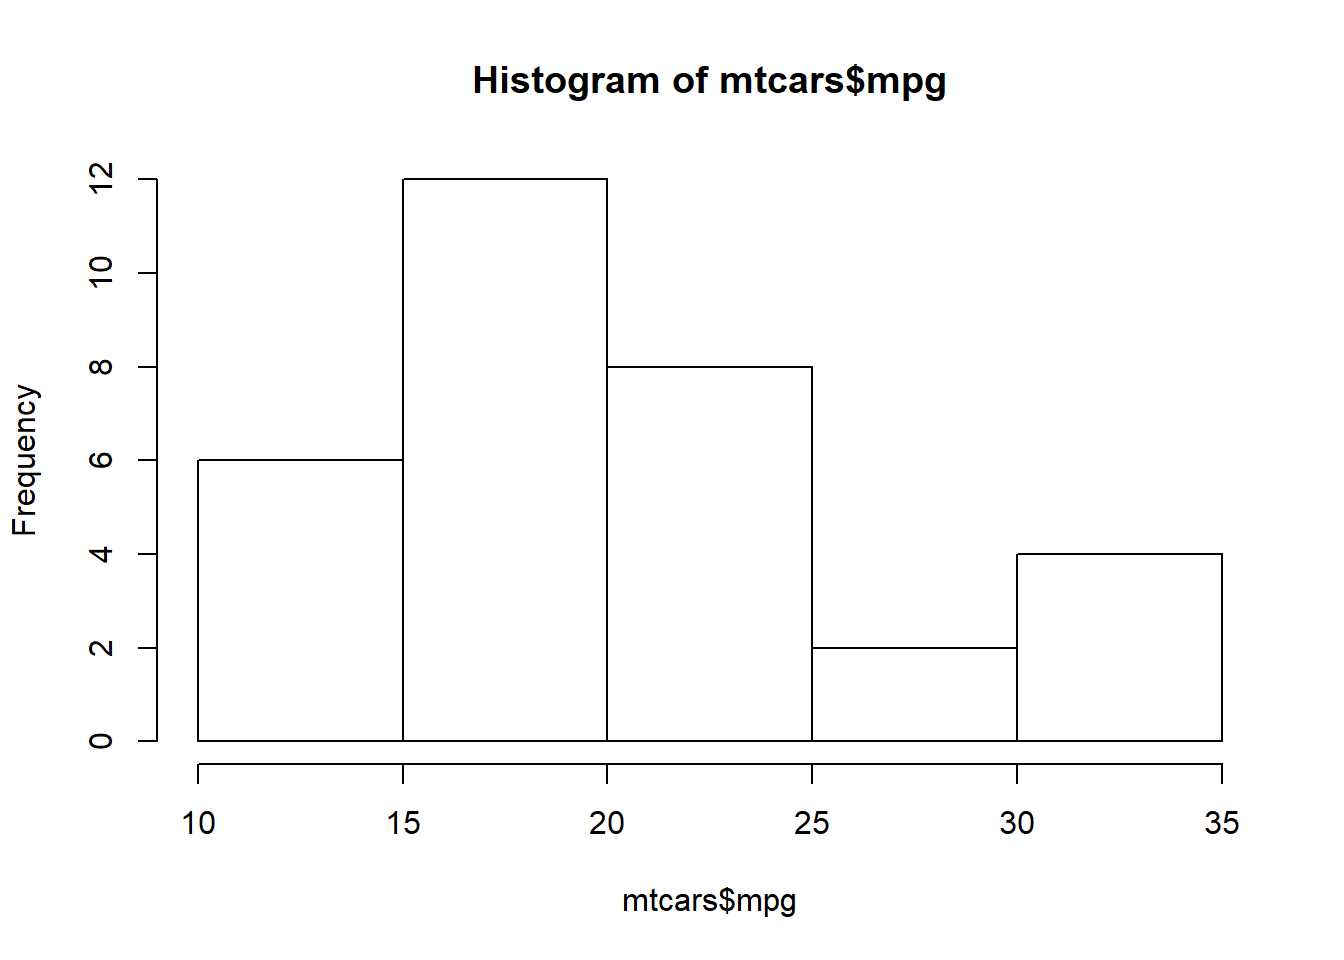
\includegraphics{bookdown_intro_files/figure-latex/figura1-1.pdf}

se generó empleando:

\begin{Shaded}
\begin{Highlighting}[]
\NormalTok{```\{r figura1, echo=FALSE\}}
\NormalTok{hist(mtcars$mpg)}
\NormalTok{```}
\end{Highlighting}
\end{Shaded}

aunque no se mostró previamente el código al haber establecido la opción
\texttt{\textasciigrave{}\textasciigrave{}\textasciigrave{}\{r,\ echo=FALSE\}}.

\subsection{Opciones de bloques de código}\label{opcodigo}

Los trozos de código pueden tener nombre y opciones, se establecen en la
cabecera de la forma
\texttt{\textasciigrave{}\textasciigrave{}\textasciigrave{}\{r\ nombre,\ op1,\ op2\}}.
Para un listado de las opciones disponibles ver
\url{http://yihui.name/knitr/options} (en la
\href{https://bookdown.org/yihui/rmarkdown/r-code.html}{Sección 2.6} del
libro de RMarkdown se incluye un resumen). En \emph{RStudio} se puede
pulsar en los iconos en la parte superior derecha del bloque de código
para establecer opciones, ejecutar todo el código anterior o sólo el
correspondiente trozo.

Algunas opciones sobre evaluación y resultados:

\begin{itemize}
\tightlist
\item
  \texttt{eval}: si \texttt{=FALSE} no se evalúa el código.
\item
  \texttt{echo}: si \texttt{=FALSE} no se muestra el código.
\item
  \texttt{include}: si \texttt{=FALSE} no se muestra el código ni ningún
  resultado.
\item
  \texttt{message,\ warning,\ error}: oculta el correspondiente tipo de
  mensaje de R (los errores o warnings se mostrarán en la consola).
\item
  \texttt{cache}: si se activa, guarda los resultados de la última
  evaluación y se reutilizan si no cambió el bloque de código (más
  detalles \href{https://yihui.name/knitr/options/\#cache}{aquí}). Puede
  ser de utilidad durante la redacción del documento para reducir el
  tiempo de renderizado (usándolo con cuidado y desactivándolo al
  terminar).
\end{itemize}

Algunas opciones sobre resultados gráficos:

\begin{itemize}
\tightlist
\item
  \texttt{fig.width,\ fig.height,\ fig.dim}: dimensiones del dispositivo
  gráfico de R (no confundir con el tamaño del resultado), e.g.
  \texttt{fig.width\ =\ 5}.
\item
  \texttt{out.width,\ out.heigh}: tamaño del gráfico, e.g.
  \texttt{=\textquotesingle{}80\%\textquotesingle{}}.
\item
  \texttt{fig.align}:
  \texttt{=\textquotesingle{}left\textquotesingle{},\ \textquotesingle{}center\textquotesingle{},\ \textquotesingle{}right\textquotesingle{}},
  establece la alineación.
\item
  \texttt{fig.cap}: leyenda de la figura\footnote{Si se genera un
    documento en PDF/LaTeX el gráfico se mostrará en un entorno flotante
    y se puede ajustar la posición empleando la opción \texttt{fig.pos}
    (por ejemplo,
    \texttt{fig.pos\ =\ \textquotesingle{}!htb\textquotesingle{}}).}.
\item
  \texttt{dev}: dispositivo gráfico de R, por defecto
  \texttt{=\textquotesingle{}pdf\textquotesingle{}} para LaTeX y
  \texttt{\textquotesingle{}png\textquotesingle{}} para HTML. Otras
  opciones son \texttt{\textquotesingle{}svg\textquotesingle{}} o
  \texttt{\textquotesingle{}jpeg\textquotesingle{}}.
\end{itemize}

Para establecer valores por defecto para todos los bloques de código se
suele incluir uno de configuración al principio del documento, por
ejemplo:

\begin{Shaded}
\begin{Highlighting}[]
\NormalTok{```\{r, setup, include=FALSE\}}
\NormalTok{knitr::opts_chunk$set(comment=NA, prompt=TRUE, dev='svg', fig.dim=c(5, 7), collapse=TRUE)}
\NormalTok{```}
\end{Highlighting}
\end{Shaded}

\section{Tablas}\label{tablas}

Las tablas en Markdown son de la forma:

\begin{verbatim}
| First Header  | Second Header |
| ------------- | ------------- |
| Row1 Cell1    | Row1 Cell2    |
| Row2 Cell1    | Row2 Cell2    |
\end{verbatim}

Por ejemplo:

\begin{longtable}[]{@{}ll@{}}
\toprule
Variable & Descripción\tabularnewline
\midrule
\endhead
mpg & Millas / galón (EE.UU.)\tabularnewline
cyl & Número de cilindros\tabularnewline
disp & Desplazamiento (pulgadas cúbicas)\tabularnewline
hp & Caballos de fuerza bruta\tabularnewline
drat & Relación del eje trasero\tabularnewline
wt & Peso (miles de libras)\tabularnewline
qsec & Tiempo de 1/4 de milla\tabularnewline
vs & Cilindros en V/Straight (0 = cilindros en V, 1 = cilindros en
línea)\tabularnewline
am & Tipo de transmisión (0 = automático, 1 = manual)\tabularnewline
gear & Número de marchas (hacia adelante)\tabularnewline
carb & Número de carburadores\tabularnewline
\bottomrule
\end{longtable}

Para convertir resultados de R en tablas de una forma simple se puede
emplear la función \texttt{ktable} del paquete \emph{knitr}. Por ejemplo
la Tabla \ref{tab:kable} se obtuvo mediante el siguiente código:

\begin{Shaded}
\begin{Highlighting}[]
\NormalTok{knitr}\OperatorTok{::}\KeywordTok{kable}\NormalTok{(}
  \KeywordTok{head}\NormalTok{(mtcars), }
  \DataTypeTok{caption =} \StringTok{"Una kable knitr"}
\NormalTok{)}
\end{Highlighting}
\end{Shaded}

\begin{table}

\caption{\label{tab:kable}Una kable knitr}
\centering
\begin{tabular}[t]{l|r|r|r|r|r|r|r|r|r|r|r}
\hline
  & mpg & cyl & disp & hp & drat & wt & qsec & vs & am & gear & carb\\
\hline
Mazda RX4 & 21.0 & 6 & 160 & 110 & 3.90 & 2.620 & 16.46 & 0 & 1 & 4 & 4\\
\hline
Mazda RX4 Wag & 21.0 & 6 & 160 & 110 & 3.90 & 2.875 & 17.02 & 0 & 1 & 4 & 4\\
\hline
Datsun 710 & 22.8 & 4 & 108 & 93 & 3.85 & 2.320 & 18.61 & 1 & 1 & 4 & 1\\
\hline
Hornet 4 Drive & 21.4 & 6 & 258 & 110 & 3.08 & 3.215 & 19.44 & 1 & 0 & 3 & 1\\
\hline
Hornet Sportabout & 18.7 & 8 & 360 & 175 & 3.15 & 3.440 & 17.02 & 0 & 0 & 3 & 2\\
\hline
Valiant & 18.1 & 6 & 225 & 105 & 2.76 & 3.460 & 20.22 & 1 & 0 & 3 & 1\\
\hline
\end{tabular}
\end{table}

Otros paquetes proporcionan opciones adicionales: \emph{xtable},
\emph{stargazer}, \emph{pander}, \emph{tables} y \emph{ascii}.

\section{Cabecera YAML}\label{yaml}

En un fichero RMarkdown se puede incluir metadatos en una cabecera en
formato YAML (YAML Ain't Markup Language,
\url{https://en.wikipedia.org/wiki/YAML}), comenzando y terminando con
tres guiones \texttt{-\/-\/-}. Los metadatos de YAML son típicamente
opciones de renderizado consitentes en pares de etiquetas y valores
separados por dos puntos\footnote{La mayoría de los campos YAML son
  opciones que el paquete \texttt{rmarkdown} le pasa a Pandoc (ver
  \url{https://pandoc.org/MANUAL.html}).}. Por ejemplo:

\begin{Shaded}
\begin{Highlighting}[]
\OtherTok{---}
\FunctionTok{title:}\AttributeTok{ }\StringTok{"Creación de contenidos con RMarkdown"}
\FunctionTok{author:}\AttributeTok{ }\StringTok{"Fernández-Casal, R. y Cotos-Yáñez, T.R."}
\FunctionTok{date:}\AttributeTok{ }\StringTok{"`r Sys.Date()`"}
\FunctionTok{output:}\AttributeTok{ html_document}
\OtherTok{---}
\end{Highlighting}
\end{Shaded}

Aunque no siempre es necesario, se recomienda que los valores de texto
se introduzcan entre comillas (se puede incluir código R en línea, como
por ejemplo \texttt{\textasciigrave{}r\ Sys.Date()\textasciigrave{}}
para obtener la fecha actual). Para valores lógicos se puede emplear
\texttt{yes/true} y \texttt{no/false} para verdadero y falso,
respectivamente.

Los valores pueden ser vectores, por ejemplo las siguientes opciones son
equivalentes:

\begin{Shaded}
\begin{Highlighting}[]
\FunctionTok{bibliography:}\AttributeTok{ }\KeywordTok{[}\NormalTok{book.bib}\KeywordTok{,}\NormalTok{ packages.bib}\KeywordTok{]}
\end{Highlighting}
\end{Shaded}

\begin{Shaded}
\begin{Highlighting}[]
\FunctionTok{bibliography:}
\KeywordTok{-}\NormalTok{ book.bib}
\KeywordTok{-}\NormalTok{ packages.bib}
\end{Highlighting}
\end{Shaded}

También pueden ser listas, añadiendo una sangría de dos espacios
(importante):

\begin{Shaded}
\begin{Highlighting}[]
\FunctionTok{output:}
  \FunctionTok{html_document:}
    \FunctionTok{toc:}\AttributeTok{ yes}
    \FunctionTok{toc_float:}\AttributeTok{ yes}
  \FunctionTok{pdf_document:}
    \FunctionTok{toc:}\AttributeTok{ yes}
\end{Highlighting}
\end{Shaded}

El campo \texttt{output} permite especificar el formato y las opciones
de salida (por defecto se empleará la primera). Empleando este campo
también se pueden especificar opciones gráficas para los bloques de
código, por ejemplo:

\begin{Shaded}
\begin{Highlighting}[]
\FunctionTok{output:}
  \FunctionTok{html_document:}
    \FunctionTok{fig_width:}\AttributeTok{ 7}
    \FunctionTok{fig_height:}\AttributeTok{ 6}
    \FunctionTok{fig_caption:}\AttributeTok{ true}
\end{Highlighting}
\end{Shaded}

La mayoría de los campos YAML son opciones que el paquete
\texttt{rmarkdown} le pasa a Pandoc (ver documentación en el Apéndice
\ref{pandoc}).

Un ejemplo adicional\footnote{Puede ser interesante ejecutar
  \texttt{str(rmarkdown::html\_document())} para ver un listado de todas
  las opciones disponibles de \texttt{html\_document}}:

\begin{Shaded}
\begin{Highlighting}[]
\OtherTok{---}
\FunctionTok{title:}\AttributeTok{ }\StringTok{"Creación de contenidos con RMarkdown"}
\FunctionTok{subtitle:}\AttributeTok{ }\StringTok{"Curso de introducción a R"}
\FunctionTok{author:}
\KeywordTok{-} \FunctionTok{name:}\AttributeTok{ }\StringTok{"Rubén Fernández Casal (ruben.fcasal@udc.es)"}
  \FunctionTok{affiliation:}\AttributeTok{ }\StringTok{"Universidade da Coruña"}
\KeywordTok{-} \FunctionTok{name:}\AttributeTok{ }\StringTok{"Tomás R. Cotos Yáñez (tcotos@uvigo.es)"}
  \FunctionTok{affiliation:}\AttributeTok{ }\StringTok{"Universidade de Vigo"}
\FunctionTok{date:}\AttributeTok{ }\StringTok{"2018-10-25"}
\FunctionTok{logo:}\AttributeTok{ rmarkdown.png}
\FunctionTok{output:}
  \FunctionTok{html_document:}
    \FunctionTok{toc:}\AttributeTok{ yes                  }\CommentTok{# incluir tabla de contenido}
    \FunctionTok{toc_float:}\AttributeTok{ yes            }\CommentTok{# toc flotante a la izquierda}
    \FunctionTok{number_sections:}\AttributeTok{ yes      }\CommentTok{# numerar secciones y subsecciones}
    \FunctionTok{code_folding:}\AttributeTok{ hide        }\CommentTok{# por defecto el código aparecerá oculto}
    \FunctionTok{mathjax:}\AttributeTok{ local            }\CommentTok{# emplea una copia local de MathJax, hay que establecer:}
    \FunctionTok{self_contained:}\AttributeTok{ false     }\CommentTok{# las dependencias se guardan en ficheros externos}
    \FunctionTok{lib_dir:}\AttributeTok{ libs             }\CommentTok{# directorio para librerías (Bootstrap, MathJax, ...)}
  \FunctionTok{pdf_document:}
    \FunctionTok{toc:}\AttributeTok{ yes}
    \FunctionTok{toc_depth:}\AttributeTok{ 2}
    \FunctionTok{keep_tex:}\AttributeTok{ yes             }\CommentTok{# conservar fichero latex}
    
\OtherTok{---}
\end{Highlighting}
\end{Shaded}

Como se puede deducir del ejemplo anterior, en el formato YAML podemos
incluir comentarios con el carácter \texttt{\#} (por ejemplo para no
emplear alguna de las opciones sin borrarla del encabezado).

En el
\href{https://bookdown.org/yihui/rmarkdown/documents.html}{Capítulo 3}
del libro de RMarkdown se tiene información detallada sobre las opciones
de los distintos formatos de salida (sobre ficheros HTML
\href{https://bookdown.org/yihui/rmarkdown/html-document.html}{aquí} y
sobre PDF/LaTeX
\href{https://bookdown.org/yihui/rmarkdown/pdf-document.html}{aquí}).

\section{Extracción del código R}\label{extraccion-del-codigo-r}

Para generar un fichero con el código R se puede emplear la función
\texttt{purl} del paquete \emph{knitr}. Por ejemplo:

\begin{verbatim}
purl("Informe.Rmd")
\end{verbatim}

Si se quiere además el texto RMarkdown como comentarios tipo
\texttt{spin}, se puede emplear:

\begin{verbatim}
purl("Informe.Rmd", documentation = 2)
\end{verbatim}

\section{Spin}\label{spin}

Una forma rápida de crear este tipo de informes a partir de un fichero
de código R es emplear la funcion \texttt{spin} del paquete \emph{knitr}
(ver p.e. \url{http://yihui.name/knitr/demo/stitch}).

Para ello se debe comentar todo lo que no sea código R de una forma
especial:

\begin{itemize}
\item
  El texto RMarkdown se comenta con \texttt{\#\textquotesingle{}}. Por
  ejemplo:

\begin{verbatim}
#' # Este es un título de primer nivel
#' ## Este es un título de segundo nivel
\end{verbatim}
\item
  Las opciones de un trozo de código se comentan con \texttt{\#+}. Por
  ejemplo:

\begin{verbatim}
#+ setup, include=FALSE
opts_chunk$set(comment=NA, prompt=TRUE, dev='svg', fig.height=6, fig.width=6)
\end{verbatim}
\end{itemize}

Para generar el informe se puede emplear la funcion \texttt{spin} del
paquete \emph{knitr}. Por ejemplo: \texttt{spin("Ridge\_Lasso.R")}.
También se podría abrir directamente el informe generado:

\begin{verbatim}
browseURL(url = knitr::spin("Ridge_Lasso.R"))
\end{verbatim}

Pero puede ser recomendable renderizarlo con rmarkdown:

\begin{verbatim}
library(rmarkdown)
browseURL(url = render(knitr::spin("Ridge_Lasso.R", knit = FALSE)))
\end{verbatim}

En \emph{RStudio} basta con pulsar ``Ctrl + Shift + K'' o seleccionar
\emph{File \textgreater{} Knit Document} (en las últimas versiones
también \emph{File \textgreater{} Compile Notebook} o hacer clic en el
icono correspondiente).

\section{Extensiones RMarkdown de
pandoc}\label{extensiones-rmarkdown-de-pandoc}

Como ya se comentó, RMarkdown utiliza la sintaxis extendida
proporcionada por Pandoc. Por ejemplo, se pueden añadir
sub\textsubscript{índices} y super\textsuperscript{índices} con
\texttt{sub\textasciitilde{}índices\textasciitilde{}} y
\texttt{super\^{}índices\^{}},\\
y notas al pie con \texttt{\^{}{[}texto{]}}.

Podemos incluir expresiones matemáticas en formato LateX:

\begin{itemize}
\item
  En linea escribiendo la expresión latex entre dos símbolos de dolar,
  por ejemplo
  \texttt{\$\textbackslash{}alpha,\ \textbackslash{}beta,\ \textbackslash{}gamma,\ \textbackslash{}delta\$}
  resultaría en \(\alpha, \beta, \gamma, \delta\).
\item
  En formato ecuación empleando dos pares de símbolos de dolar. Por
  ejemplo:

\begin{verbatim}
$$\Theta = \begin{pmatrix}\alpha & \beta\\
\gamma & \delta
\end{pmatrix}$$
\end{verbatim}

  resultaría en: \[\Theta = \begin{pmatrix}\alpha & \beta\\
  \gamma & \delta
  \end{pmatrix}\]
\end{itemize}

También admite bibliografía, ver p.e.
\url{https://rmarkdown.rstudio.com/authoring_bibliographies_and_citations.html}.
Lo más cómodo puede ser emplear un archivo de bibliografía en formato
BibTeX, lo que se describe con detalle
\href{https://bookdown.org/yihui/bookdown/citations.html}{aquí}. Será
necesario añadir un campo \texttt{bibliography} en la cabezera YAML, por
ejemplo:

\begin{Shaded}
\begin{Highlighting}[]
\FunctionTok{bibliography:}\AttributeTok{ bibliografia.bib}
\FunctionTok{csl:}\AttributeTok{ apa.csl  }\CommentTok{# opcional}
\end{Highlighting}
\end{Shaded}

Suponiendo que en el directorio de trabajo están los ficheros de
bibliografía \emph{bibliografia.bib} y de estilo \emph{apa.csl} (ver
\url{http://citationstyles.org/}, desde donde se pueden descargar
distintos archivos de estilo).

Las referencias en el texto RMarkdown se incluyen con
\texttt{@referencia} o \texttt{{[}@referencia{]}}. Pandoc generará el
listado de referencias al final del documento, por lo que nos puede
interesar insertar una última sección \texttt{\#\ Referencias\ \{-\}} al
generar documentos HTML (en PDF se hará automáticamente al emplear
LaTeX). En RStudio se puede instalar el
``\href{https://rstudio.github.io/rstudioaddins/}{Addin}''
\href{https://github.com/crsh/citr}{\texttt{citr}} para insertar citas a
referencias bibliográficas en formato BibTeX.

Para más detalles de las extensiones de Pandoc ver por ejemplo
\url{https://rmarkdown.rstudio.com/authoring_pandoc_markdown.html\%23raw-tex}
o el manual de Pandoc \url{https://pandoc.org/MANUAL.html}.

\chapter{Pandoc}\label{pandoc}

\section{Introducción}\label{introduccion-2}

Pandoc es un conversor de documentos libre y de código abierto, Pandoc
puede leer archivos en distintos formatos, incluyendo:

\begin{itemize}
\item
  Distintos dialectos de
  \href{http://daringfireball.net/projects/markdown/}{Markdown}
\item
  \href{http://www.w3.org/TR/html40/}{HTML}
\item
  \href{http://www.latex-project.org/}{LaTeX}
\item
  Microsoft Word
  \href{https://en.wikipedia.org/wiki/Office_Open_XML}{docx}
\item
  LibreOffice \href{http://en.wikipedia.org/wiki/OpenDocument}{ODT}
\item
  \href{http://en.wikipedia.org/wiki/EPUB}{EPUB}
\end{itemize}

Puede convertir los documentos de entrada a muchos otros formatos,
incluyendo Office Open XML, OpenDocument, HTML, Wiki markup, InDesign
ICML, ebooks, OPML, y varios formatos basados en TeX (desde donde se
puede producir un PDF). En la web oficial \url{https://pandoc.org} hay
un listado completo de los formatos soportados. Pandoc también
proporciona distintas extensiones de Markdown para que admita resultados
más complejos.

Pandoc es una herramienta independiente de línea de comandos (sin
interfaz gráfica), que se instala automáticamente con RStudio porque el
paquete \texttt{rmarkdown} la emplea para generar los documentos de
salida a partir de documentos Markdown (por ejemplo, en Windows en
\emph{C:\textbackslash{}Program
Files\textbackslash{}RStudio\textbackslash{}bin\textbackslash{}pandoc\textbackslash{}pandoc.exe}).

\section{Conversión de documentos con Pandoc}\label{conversion}

La sintaxis del comando es
\texttt{pandoc\ {[}opciones{]}\ {[}ficheros{]}}. Si se ejecuta
\texttt{pandoc\ -\/-help}, en la ventana de comandos o en la pestaña
\emph{Terminal} de RStudio, se obtiene un listado detallado de las
opciones. También se puede consultar el manual de Pandoc
\url{https://pandoc.org/MANUAL.html}.

Si Pandoc no está configurado en la ruta de búsqueda, habrá que
reemplazar \texttt{pandoc} por la ruta completa al ejecutable. Por
ejemplo, para emplear la versión instalada con RStudio en Windows habra
que introducir
\texttt{"C:\textbackslash{}Program\ Files\textbackslash{}RStudio\textbackslash{}bin\textbackslash{}pandoc\textbackslash{}pandoc"}.

Podemos emplear Pandoc para convertir contenido escrito en otros
formatos a Markdown, por ejemplo:

\begin{itemize}
\item
  Un fichero word a markdown

\begin{verbatim}
"C:\Program Files\RStudio\bin\pandoc\pandoc" fichero.docx -f docx -t markdown 
--extract-media . -o fichero.Rmd 
\end{verbatim}
\item
  Un fichero LaTeX a markdown

\begin{verbatim}
"C:\Program Files\RStudio\bin\pandoc\pandoc" fichero.tex -f latex -t markdown 
-o fichero.Rmd 
\end{verbatim}
\item
  Una web a markdown

\begin{verbatim}
"C:\Program Files\RStudio\bin\pandoc\pandoc" http://url.org -f html -t markdown 
-o fichero.Rmd
\end{verbatim}
\end{itemize}

Por defecto \emph{pandoc} produce en algunos casos un fragmento de
documento (cuando el formato de salida no es markdown). Para obtener un
documento independiente (e.g.~un fichero HTML válido incluyendo
\texttt{\textless{}head\textgreater{}} y
\texttt{\textless{}body\textgreater{}}), habrá que emplear la opción
\texttt{-s} o \texttt{-\/-standalone}.

\section{Pandoc y RMarkdown}\label{pandoc-y-rmarkdown}

Como ya se comentó, el paquete \texttt{rmarkdown} llama a \emph{pandoc}
para renderizar un documento RMarkdown\footnote{Desde la
  \href{https://blog.rstudio.org/2014/06/18/r-markdown-v2/}{versión 2},
  antes se utilizaba \texttt{knitr} y \texttt{markdown}.}, y esta
llamada se muestra en la consola (o en la correspondiente pestaña de
RStudio):

\begin{verbatim}
"C:/Program Files/RStudio/bin/pandoc/pandoc" +RTS -K512m -RTS Informes.utf8.md --to html4 
--from markdown+autolink_bare_uris+ascii_identifiers+tex_math_single_backslash 
--output Informes.html --smart --email-obfuscation none --self-contained --standalone 
--section-divs --table-of-contents --toc-depth 3 --variable toc_float=1 
--variable toc_selectors=h1,h2,h3 --variable toc_collapsed=1 --variable toc_smooth_scroll=1 
--variable toc_print=1 --template "C:\PROGRA~1\R\R-35~1.1\library\RMARKD~1\rmd\h\DEFAUL~1.HTM"
--no-highlight --variable highlightjs=1 --variable "theme:bootstrap" --include-in-header
"C:\Users\RUBEN~1.FCA\AppData\Local\Temp\RtmpkntXD8\rmarkdown-str2084caf51da.html" --mathjax 
--variable "mathjax-url:https://mathjax.rstudio.com/latest/MathJax.js?config=TeX-AMS-MML_HTMLorMML"

Output created: Informes.html
\end{verbatim}

La mayoría de los campos de la cabecera YAML de un fichero RMarkdown se
traducen en las opciones de Pandoc. Por ejemplo, la cabezera:

\begin{Shaded}
\begin{Highlighting}[]
\OtherTok{---}
\FunctionTok{output:}
  \FunctionTok{html_document:}
    \FunctionTok{number_sections:}\AttributeTok{ yes      }
\OtherTok{---}
\end{Highlighting}
\end{Shaded}

(que produce la numeración de secciones y subsecciones), se corresponde
con la opción \texttt{-\/-number-sections} de \emph{pandoc}. También se
puede establecer cualquier opción de Pandoc en la cabecera YAML mediante
el campo \texttt{pandoc\_args}, por ejemplo:

\begin{Shaded}
\begin{Highlighting}[]
\OtherTok{---}
\FunctionTok{output:}
  \FunctionTok{html_document:}\AttributeTok{ }
    \FunctionTok{pandoc_args:}\AttributeTok{ }\KeywordTok{[}\StringTok{"--number-offset"}\KeywordTok{,} \StringTok{"4,0"}\KeywordTok{,} \StringTok{"--number-sections"}\KeywordTok{]}\AttributeTok{      }
\OtherTok{---}
\end{Highlighting}
\end{Shaded}

(en este caso la numeración comenzaría en 4).

\bibliography{book.bib,packages.bib}


\end{document}
